\documentclass{article}
\usepackage[T2A]{fontenc}
\usepackage[english,russian]{babel}
\usepackage[utf8]{inputenc}
% \usetheme{Warsaw}
\usepackage{graphics}
\usepackage{graphicx}
\graphicspath{ {./images/} }
\usepackage{subfig}
\usepackage[utf8]{inputenc}
\usepackage{amsmath, amssymb}
\usepackage[export]{adjustbox}

\title{Отчёт о проделанной работе}
\author{Лазар В. И.}
\date{12.11.2024}

\begin{document}
\maketitle

\section{Проведённые исследования}

\subsection{Модель}

Программно реализована однопиковая модель \textbf{PBFTPK} с возможностью обучения на данных и генерации сэмплов с параметрами, подобранными при обучении. \newline

Сама модель устроена следующим образом:

$$
	C(t) = \begin{cases}
		\frac{F D k_a}{V_d (k_a - k_{el})} (e^{-k_{el} t} - e^{-k_a t}), t \le \tau \\
		C(\tau)e^{-k_el (t - \tau)}, t > \tau
	\end{cases}
$$
\begin{align*}
	 & C(t) - \text{концентрация декарства в крови}                     \\
	 & D > 0 - \text{объём дозы лекарства}                              \\
	 & F > 0 - \text{биодоступная доля дозы}                            \\
	 & V_d > 0 - \text{объём распределения лекарства}                   \\
	 & k_a - \text{параметр всасывания вещества}                        \\
	 & k_el - \text{параметр выведения вещества}                        \\
	 & \tau > 0 - \text{время абсорбции}, C(\tau) = \sup_{t \ge 0} C(t)
\end{align*}


\subsection{Метрика}

В качестве метрики для оценки моделей большинство уже реализованных алгоритмов используют метрику \[
	\frac{1}{n}\sum_{i=1}^{n} (f(t_i) - X(t_i))^2
\], которая мало подходит в задачах биоэквивалентности в силу слабой интерпретируемости. Был реализован аналог алгоритма подбора параметров модели для метрики
\[
	\frac{1}{n}\sum_{i=1}^{n} |f(t_i) - X(t_i)|
\], что дало большее качество при обучени модели.


\subsection{Исследование моментных характеристик остатков}

Здесь и далее будем действовать в предположении о том, что величина
\[
	X(t) - f(t)
\], где X(t) - исходный случайный процесс, а f(t) - тректория предсказанная моделью, является процессом Леви

Для получения более точного вида процесса было решено исследовать матожидание и стандартное отклонение проекций процесса остатков \newline\newline


Получен следующий график поведения для матожидания

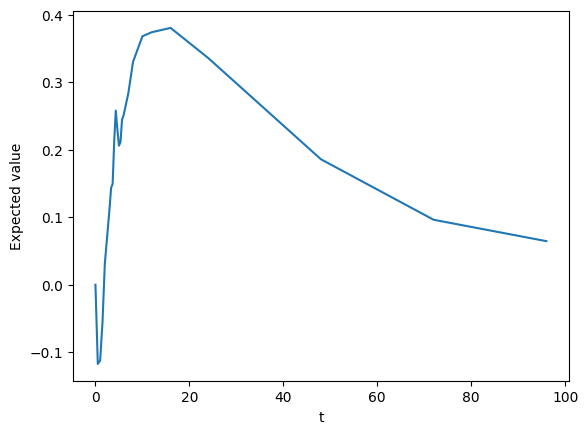
\includegraphics[width=0.7\textwidth, left]{mean.png}

И для стандартного отклонения

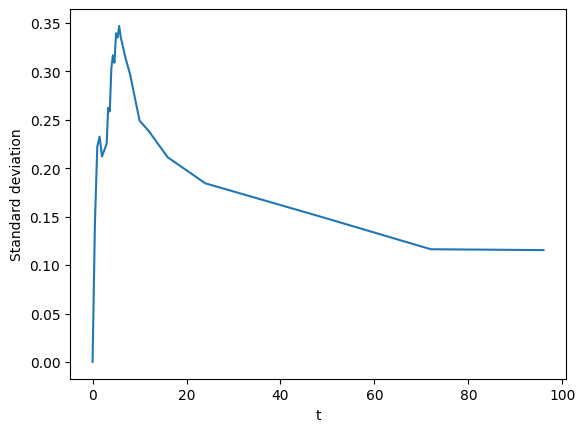
\includegraphics[width=0.7\textwidth, left]{std.png}

Заметно, что в среднем наша модель сильнее всего ошибается в окрестности 20-и. Запомним это и рассмотрим несколько графиков процессов

\subsection{Исследование поведения исходного процесса}

Здесь показаны одни из типовых случаев процессов, на которых моделm значительно ошибается ошибается

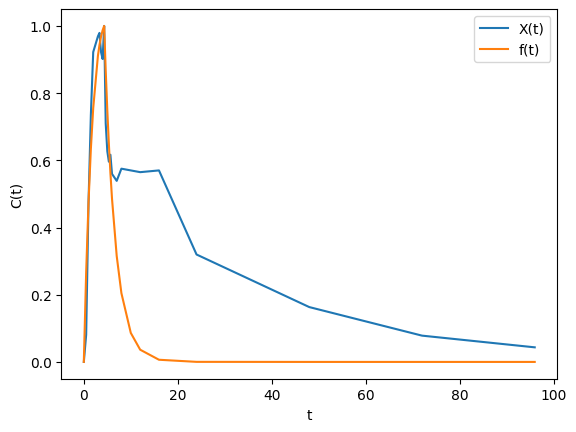
\includegraphics[width=0.7\textwidth, left]{example4.png}
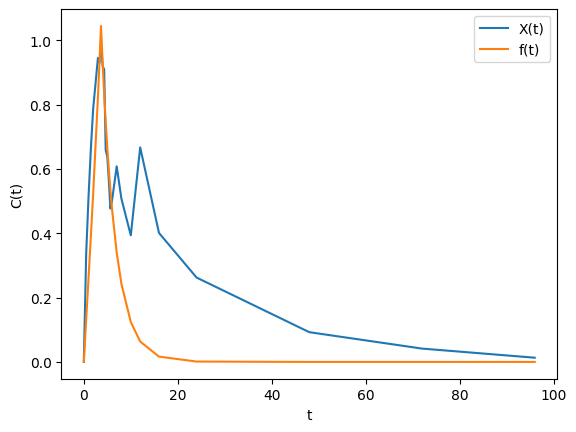
\includegraphics[width=0.7\textwidth, left]{example5.png}
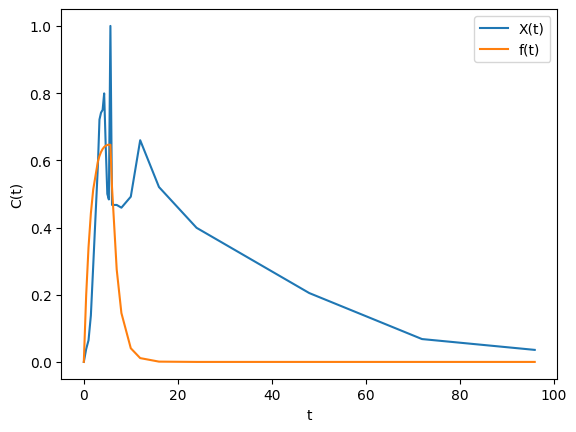
\includegraphics[width=0.7\textwidth, left]{example6.png}

Заметим, что второй пик здесь находится в окрестности 20, что согласуется с полученными выше результатами. Поскольку подобных процессов в датасете достаточно много, логично предположить, что однопиковой модели \textbf{PBFTPK} будет недостаточно для предсказания поведения процесса. Более того, учитывая, что однопиковых процессов в датасете также много, возможно логично будет предположение о небиоэквивалентности реферрентного и тестового препаратов

\section{Гипотезы и планы}

\subsection{Разметка датасета}

Поскольку была обнаружена особенность сильно влияющая на работу модели, появилась идея вручную разметить датасет и для каждого процесса указать возможное количество максимумов (от 1 до 3). Возможно, имеет смысл создать алгоритм (или обучить отдельную модель) для поиска количества пиков процесса и оценки вероятности того, что количество пиков найдено верно

\subsection{Модель}

По этой же причине было принято решение усовершенствовать модель для учёта возможных многопиковых случаев. Возможно также имеет смысл изменить функцию потерь на следующую:
\begin{align*}
	 & L(f, \alpha) = \frac{1}{n}\sum_{i=1}^{i_0-1} |f(t_i) - X(t_i)| +
	\frac{1}{n}\sum_{i=i_0}^{n} \alpha|f(t_i) - X(t_i)|                 \\
	 & \alpha \ge 0                                                     \\
	 & X(t_i) = \tau
\end{align*}

Коэффициент $\alpha$ отвечает за то, насколько сильно на общую ошибку влияет отклонение после времени абсорбции $\tau$. Это может быть полезным, так как сильнее всего модель ошибается после  достижения пика.

\end{document}
